%!TEX root=../document.tex

\section{Ergebnisse}
\label{sec:Ergebnisse}
	
\subsection{Tests Allgemein}
Zu den allgemeinen Tests zählten hier Konversionen der Brüche in Integer, Float und so weiter.
Dazu kann man sich, wie bei fast allen anderen Testfällen auch, die Paramterüberschreibung von
Python zunutze machen. Konkret hei{\ss}t dass, es werden Funktionen wie zum Beispiel \_\_float\_\_
überschrieben. Auch die verwendeten Operatoren wie +, -, usw. können über die zugehörigen Methoden 
übeschrieben werden. Um Fehler bei jeweiligen Konversionen und Operationen aufzudecken, werden
Exceptions mittels 'raise' geworfen. 
Auch interessant ist der im Konstruktor verwendete Standartwert für denom, da man sonst keine Brüche
mit nur einem Zähler als Input erzeugen könnte.
Aus Gründen des Platzes ist es sinnlos den Code hier anzuzeigen, da dieser durch Kommentare sehr bloated wurde, daher zeige ich hier die Testergebnisse.

\begin{figure}[!h]
	\begin{center}
		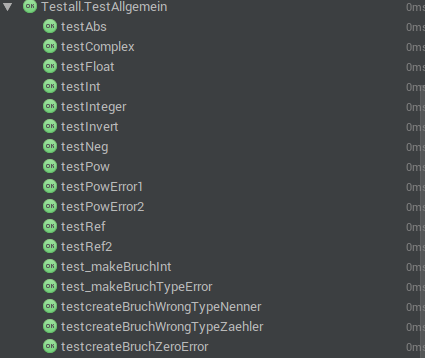
\includegraphics[width=0.6\linewidth]{images/testAllgemein.png}
		\caption{Test Allgemein}
		\label{broker}
	\end{center}
\end{figure}
\clearpage

\subsection{Vergleichs Teste}
Der Vorgang ist auch hier derselbe wie bei dem vorherigen Testgebiet, also werde ich keine lange, sinnlose Erklärung anhängen.

\begin{figure}[!h]
	\begin{center}
		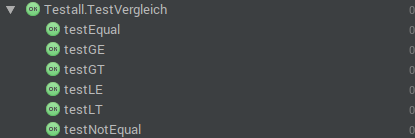
\includegraphics[width=0.6\linewidth]{images/testV.png}
		\caption{Test Allgemein}
		\label{broker}
	\end{center}
\end{figure}

\subsection{String und Iteration}
Da diese beiden jeweils nur eine Methode umfassen, schreibe ich sie hier gemeinsam an. Die Iteration ist relativ selbserklärend. Die String Methonden sind anzusehen wie toString in Java. Ich habe mir hier einfach String Templates zunutze gemacht um die Werte in String einzufüllen und diese zu returnen. Man muss hierbei aber auch wieder auf Sonderfälle wie ganze Brüche achten. Diese werden nämlich in ihrer Integer Form dargestellt.

\begin{figure}[!h]
	\begin{center}
		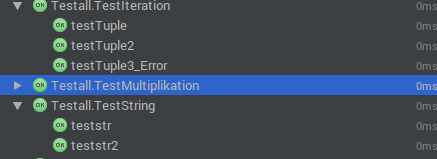
\includegraphics[width=0.6\linewidth]{images/testB.png}
		\caption{Test Iteration und Strings}
		\label{broker}
	\end{center}
\end{figure}


\clearpage

\subsection{Addition und Subtraktion}
Da diese dasselbe Prinzip verfolge, werden sie zusammengefasst. Wieder mittels der Überschreibung von passenden Funktionen, kann man die Addition und Subtraktion von Brüchen mit Integern, sowie mit anderen Brüchen ermöglichen. Hierbei muss aber immer dass kleinste gemeinsame Vielfache als Wert des Nenners für die neuen Brüche beachtet werden. Damit die Subtraktion nicht extra implementiert werden musste, habe ich einfach die Additionsfunktion hier auch benutzt um mit einem negativen Wert zu addieren.

\begin{figure}[!h]
	\begin{center}
		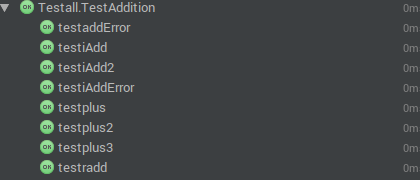
\includegraphics[width=0.6\linewidth]{images/testAdd.png}
		\caption{Test Addition}
		\label{broker}
	\end{center}
\end{figure}

\begin{figure}[!h]
	\begin{center}
		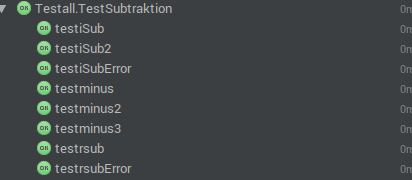
\includegraphics[width=0.6\linewidth]{images/testSub.png}
		\caption{Test Subktraktion}
		\label{broker}
	\end{center}
\end{figure}
\clearpage

\subsection{Multiplikation und Division}
Verfolgen das selbe Prinzip wie der Code von Addition und Subtraktion, daher sind diese auch gleich aufgebaut, nur mit den jeweils passenden Überschreibungen versehen. Man muss hier aber aufpassen, dass einem keine Division durch 0 untergerät, daher werden hier häufiger Checks durchgeführt. Auch beim Kreuzprodukt bei der Multiplikation und bei dem Doppelbruch der Division muss man auf jeweilige Sonderfälle aufpasse.

\begin{figure}[!h]
	\begin{center}
		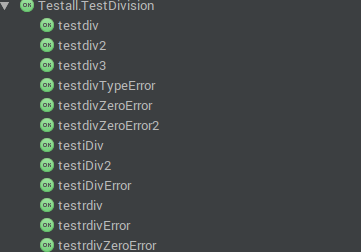
\includegraphics[width=0.6\linewidth]{images/testDiv.png}
		\caption{Test Divison}
		\label{broker}
	\end{center}
\end{figure}
\begin{figure}[!h]
	\begin{center}
		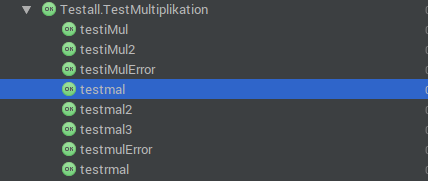
\includegraphics[width=0.6\linewidth]{images/testMul.png}
		\caption{Test Multiplikation}
		\label{broker}
	\end{center}
\end{figure}
\clearpage

\subsection{Code Coverage}
Anhand der Testreports im doku Ordner wird erkennt man gut, das die erforderlichen 95\% erreicht wurden.
Hier anbei aber noch einmal ein Screenshot der PyCharm Ausgabe.

\begin{figure}[!h]
	\begin{center}
		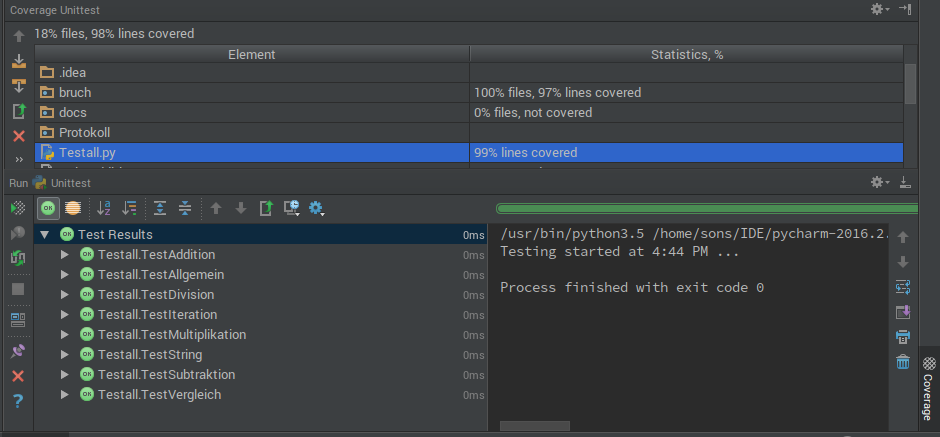
\includegraphics[width=0.9\linewidth]{images/coverage.png}
		\caption{Test Coverage}
		\label{broker}
	\end{center}
\end{figure}


